\documentclass[12pt,a4paper]{article}
\usepackage[utf8]{inputenc}
\usepackage[spanish]{babel}
\usepackage{amsmath}
\usepackage{amsfonts}
\usepackage{amssymb}
\usepackage{graphicx}
\author{Manuel González González}
\title{Práctica 9: Detección de Movimiento}
\begin{document}
\maketitle

\section*{Ejercicio 2}
\subsection*{a)}
En la primera imagen se puede ver el ejemplo de eta=1 y en la segunda eta=0.4.

Cuando eta vale uno el modelo de fondo se ajusta más rápido al fondo real, esto se debe a que aprende con mayor velocidad lo que hay en los frames, o por el contrario, cuando vale 0.4 tarda más en olvidar patrones que no pertenecen al modelo de fondo.

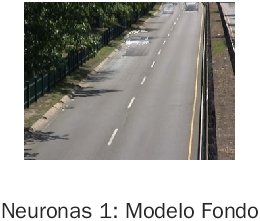
\includegraphics[scale=1]{EtaUno.png}
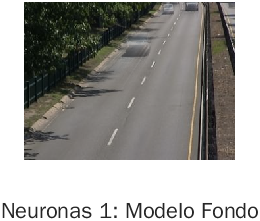
\includegraphics[scale=1]{EtaCeroCuatro.png}

\subsection*{b)}
La red no es capaz de recrear bien el modelo de fondo y por ello la segmentación no muestra la representación esperada del objeto dinámico. Esto ocurre porque la red no tiene un registro fiable del modelo de fondo, ya que al no tener una cuenta de las veces que ha ganado una neurona, no tiene capacidad de comparar fotogramas distintos.

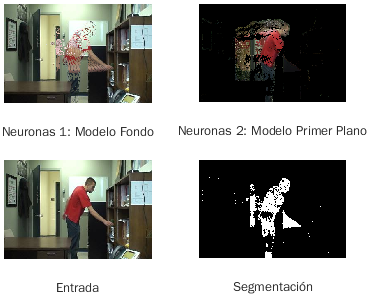
\includegraphics[scale=1]{numGanaUno.png}

\end{document}